\documentclass[12pt]{standalone}

\usepackage{tikz}

\usetikzlibrary{fadings,shapes.arrows,shadows}   
% \usetikzlibrary{shapes.geometric, shapes, arrows} 

% \renewcommand{\textwidth}{1}

\begin{document}

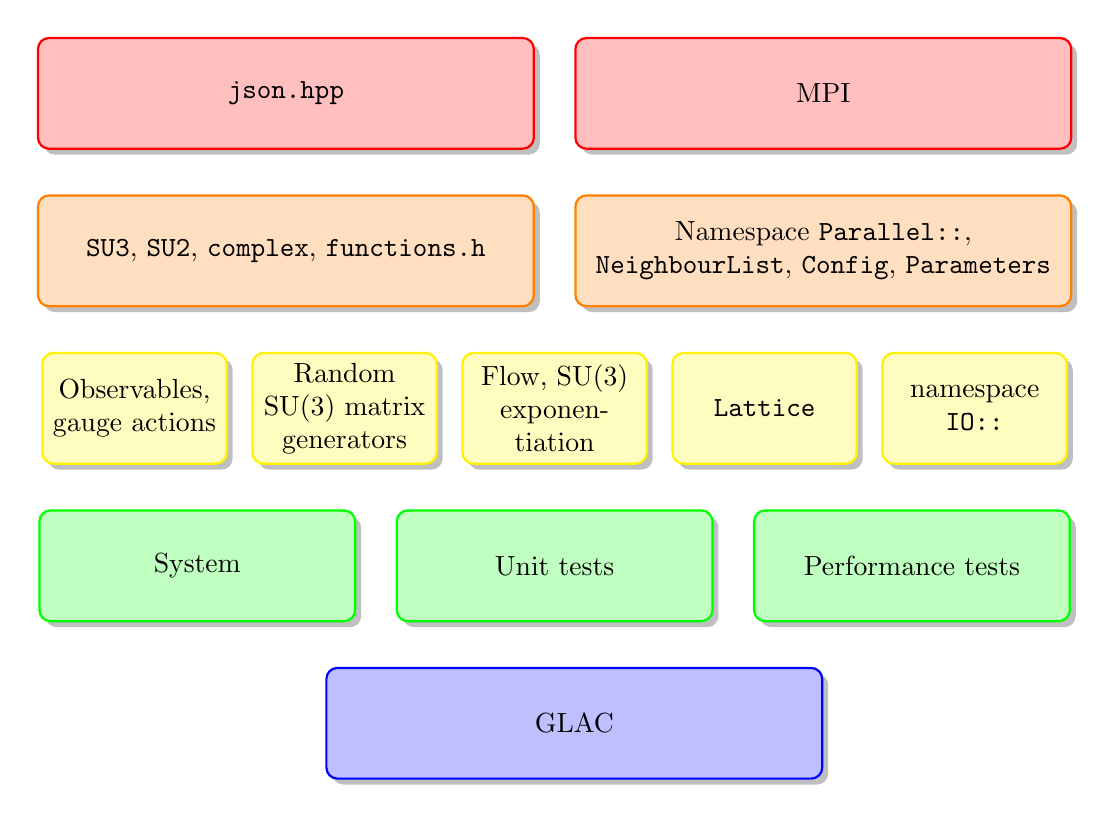
\begin{tikzpicture}
    [auto,
    % Base style
    base/.style={rectangle, draw=red, fill=red!25, thick, align=center, rounded corners, minimum height=4em, drop shadow},
    % Standalone/first derived classes
    derivedFirst/.style={rectangle, draw=orange, fill=orange!25, thick, align=center, rounded corners, minimum height=4em, drop shadow},
    % Classes using derived functionality
    derivedSecond/.style={rectangle, draw=yellow, fill=yellow!25, thick, align=center, rounded corners, minimum height=4em, drop shadow},
    % Further derived functionality
    block4/.style={rectangle, draw=green, fill=green!25, thick, align=center, rounded corners, minimum height=4em, drop shadow},
    % Final apps
    apps/.style={rectangle, draw=blue, fill=blue!25, thick, align=center, rounded corners, minimum height=4em, drop shadow},
    line/.style={draw, thick, -latex',shorten >=2pt}]
    % Base layer
    \matrix [column sep=5mm,row sep=7mm] (row0) {
       % row 1
        \node  [base, text width=\textwidth/2] (json)      {\texttt{json.hpp}}; 
        &\node [base, text width=\textwidth/2] (mpi)       {MPI};  \\ 
    };
    % Standalone/self contained modules or depends only on external functionality
    \matrix [column sep=5mm,row sep=7mm, below of=row0, yshift=-1cm] (row1){
        % row 2
        \node  [derivedFirst, text width=\textwidth/2] (math)      {\texttt{SU3}, \texttt{SU2}, \texttt{complex}, \texttt{functions.h}}; 
        &\node [derivedFirst, text width=\textwidth/2] (io)         {Namespace \texttt{Parallel::}, \texttt{NeighbourList}, \texttt{Config}, \texttt{Parameters}}; \\
    };
    % Modules dependent on previous layer(s)
    \matrix [column sep=3mm,row sep=7mm, below of=row1, yshift=-1cm] (row2) {
        % row 3
        \node  [derivedSecond, text width=\textwidth/5-3.2mm] (obs-act)       {Observables, gauge actions};
        &\node [derivedSecond, text width=\textwidth/5-3.2mm] (derivedMath)    {Random $\mathrm{SU}(3)$ matrix generators};
        &\node [derivedSecond, text width=\textwidth/5-3.2mm] (flow)    {Flow, $\mathrm{SU}(3)$ exponentiation};
        &\node [derivedSecond, text width=\textwidth/5-3.2mm] (lattice)    {\texttt{Lattice}};
        &\node [derivedSecond, text width=\textwidth/5-3.2mm] (io)    {namespace \texttt{IO::}}; \\
    };
    % Moduels that is heavily dependent on previous layers
    \matrix [column sep=5mm,row sep=7mm, below of=row2, yshift=-1cm] (row3) {
        % programs
        \node [block4, text width=\textwidth/3-2.66mm] (system)      {System};
        & \node [block4, text width=\textwidth/3-2.66mm] (unittests)      {Unit tests};
        &\node [block4, text width=\textwidth/3-2.66mm] (perftests)      {Performance tests}; \\
    };
    % Final app.
    \matrix [column sep=5mm,row sep=7mm, below of=row3, yshift=-1cm] (row4) {
        % apps
        &\node [apps, text width=\textwidth/2] (glac)      {GLAC}; \\
    };
\end{tikzpicture}


% \tikzset{
%     base/.style = {rectangle, rounded corners, draw=black,
%                            minimum width=4cm, minimum height=1cm,
%                            text centered, font=\sffamily},
%     baseLevel/.style = {base, fill=red!25},
%     derivedFirst/.style = {base, fill=orange!25},
%     derivedSecond/.style = {base, fill=yellow!25},
%     App/.style = {base, fill=blue!25},
% }


% \begin{tikzpicture}[align=center]
%     % Base level libraries
%     \node (json) [baseLevel] {\texttt{json.hpp}};
%     \node (mpi) [baseLevel, right of =json, xshift=4cm] {\texttt{MPI.h}};
%     % \node (baseArrow) [arrowstyle=fancy] {};
%     % Math, generators, Parallel
%     % Actions, observables, 
% \end{tikzpicture}

\end{document}
